% Options for packages loaded elsewhere
\PassOptionsToPackage{unicode}{hyperref}
\PassOptionsToPackage{hyphens}{url}
\PassOptionsToPackage{dvipsnames,svgnames,x11names}{xcolor}
%
\documentclass[
  10pt,
  ignorenonframetext,
  aspectratio=169,
  10pt]{beamer}
\usepackage{pgfpages}
\setbeamertemplate{caption}[numbered]
\setbeamertemplate{caption label separator}{: }
\setbeamercolor{caption name}{fg=normal text.fg}
\beamertemplatenavigationsymbolsempty
% Prevent slide breaks in the middle of a paragraph
\widowpenalties 1 10000
\raggedbottom
\setbeamertemplate{part page}{
  \centering
  \begin{beamercolorbox}[sep=16pt,center]{part title}
    \usebeamerfont{part title}\insertpart\par
  \end{beamercolorbox}
}
\setbeamertemplate{section page}{
  \centering
  \begin{beamercolorbox}[sep=12pt,center]{part title}
    \usebeamerfont{section title}\insertsection\par
  \end{beamercolorbox}
}
\setbeamertemplate{subsection page}{
  \centering
  \begin{beamercolorbox}[sep=8pt,center]{part title}
    \usebeamerfont{subsection title}\insertsubsection\par
  \end{beamercolorbox}
}
\AtBeginPart{
  \frame{\partpage}
}
\AtBeginSection{
  \ifbibliography
  \else
    \frame{\sectionpage}
  \fi
}
\AtBeginSubsection{
  \frame{\subsectionpage}
}
\usepackage{amsmath,amssymb}
\usepackage{lmodern}
\usepackage{iftex}
\ifPDFTeX
  \usepackage[T1]{fontenc}
  \usepackage[utf8]{inputenc}
  \usepackage{textcomp} % provide euro and other symbols
\else % if luatex or xetex
  \usepackage{unicode-math}
  \defaultfontfeatures{Scale=MatchLowercase}
  \defaultfontfeatures[\rmfamily]{Ligatures=TeX,Scale=1}
\fi
\usetheme[]{Frankfurt}
\usecolortheme{spruce}
\usefonttheme{professionalfonts}
% Use upquote if available, for straight quotes in verbatim environments
\IfFileExists{upquote.sty}{\usepackage{upquote}}{}
\IfFileExists{microtype.sty}{% use microtype if available
  \usepackage[]{microtype}
  \UseMicrotypeSet[protrusion]{basicmath} % disable protrusion for tt fonts
}{}
\makeatletter
\@ifundefined{KOMAClassName}{% if non-KOMA class
  \IfFileExists{parskip.sty}{%
    \usepackage{parskip}
  }{% else
    \setlength{\parindent}{0pt}
    \setlength{\parskip}{6pt plus 2pt minus 1pt}}
}{% if KOMA class
  \KOMAoptions{parskip=half}}
\makeatother
\usepackage{xcolor}
\newif\ifbibliography
\usepackage{color}
\usepackage{fancyvrb}
\newcommand{\VerbBar}{|}
\newcommand{\VERB}{\Verb[commandchars=\\\{\}]}
\DefineVerbatimEnvironment{Highlighting}{Verbatim}{commandchars=\\\{\}}
% Add ',fontsize=\small' for more characters per line
\newenvironment{Shaded}{}{}
\newcommand{\AlertTok}[1]{\textcolor[rgb]{1.00,0.00,0.00}{\textbf{#1}}}
\newcommand{\AnnotationTok}[1]{\textcolor[rgb]{0.38,0.63,0.69}{\textbf{\textit{#1}}}}
\newcommand{\AttributeTok}[1]{\textcolor[rgb]{0.49,0.56,0.16}{#1}}
\newcommand{\BaseNTok}[1]{\textcolor[rgb]{0.25,0.63,0.44}{#1}}
\newcommand{\BuiltInTok}[1]{\textcolor[rgb]{0.00,0.50,0.00}{#1}}
\newcommand{\CharTok}[1]{\textcolor[rgb]{0.25,0.44,0.63}{#1}}
\newcommand{\CommentTok}[1]{\textcolor[rgb]{0.38,0.63,0.69}{\textit{#1}}}
\newcommand{\CommentVarTok}[1]{\textcolor[rgb]{0.38,0.63,0.69}{\textbf{\textit{#1}}}}
\newcommand{\ConstantTok}[1]{\textcolor[rgb]{0.53,0.00,0.00}{#1}}
\newcommand{\ControlFlowTok}[1]{\textcolor[rgb]{0.00,0.44,0.13}{\textbf{#1}}}
\newcommand{\DataTypeTok}[1]{\textcolor[rgb]{0.56,0.13,0.00}{#1}}
\newcommand{\DecValTok}[1]{\textcolor[rgb]{0.25,0.63,0.44}{#1}}
\newcommand{\DocumentationTok}[1]{\textcolor[rgb]{0.73,0.13,0.13}{\textit{#1}}}
\newcommand{\ErrorTok}[1]{\textcolor[rgb]{1.00,0.00,0.00}{\textbf{#1}}}
\newcommand{\ExtensionTok}[1]{#1}
\newcommand{\FloatTok}[1]{\textcolor[rgb]{0.25,0.63,0.44}{#1}}
\newcommand{\FunctionTok}[1]{\textcolor[rgb]{0.02,0.16,0.49}{#1}}
\newcommand{\ImportTok}[1]{\textcolor[rgb]{0.00,0.50,0.00}{\textbf{#1}}}
\newcommand{\InformationTok}[1]{\textcolor[rgb]{0.38,0.63,0.69}{\textbf{\textit{#1}}}}
\newcommand{\KeywordTok}[1]{\textcolor[rgb]{0.00,0.44,0.13}{\textbf{#1}}}
\newcommand{\NormalTok}[1]{#1}
\newcommand{\OperatorTok}[1]{\textcolor[rgb]{0.40,0.40,0.40}{#1}}
\newcommand{\OtherTok}[1]{\textcolor[rgb]{0.00,0.44,0.13}{#1}}
\newcommand{\PreprocessorTok}[1]{\textcolor[rgb]{0.74,0.48,0.00}{#1}}
\newcommand{\RegionMarkerTok}[1]{#1}
\newcommand{\SpecialCharTok}[1]{\textcolor[rgb]{0.25,0.44,0.63}{#1}}
\newcommand{\SpecialStringTok}[1]{\textcolor[rgb]{0.73,0.40,0.53}{#1}}
\newcommand{\StringTok}[1]{\textcolor[rgb]{0.25,0.44,0.63}{#1}}
\newcommand{\VariableTok}[1]{\textcolor[rgb]{0.10,0.09,0.49}{#1}}
\newcommand{\VerbatimStringTok}[1]{\textcolor[rgb]{0.25,0.44,0.63}{#1}}
\newcommand{\WarningTok}[1]{\textcolor[rgb]{0.38,0.63,0.69}{\textbf{\textit{#1}}}}
\usepackage{longtable,booktabs,array}
\usepackage{calc} % for calculating minipage widths
\usepackage{caption}
% Make caption package work with longtable
\makeatletter
\def\fnum@table{\tablename~\thetable}
\makeatother
\usepackage{graphicx}
\makeatletter
\def\maxwidth{\ifdim\Gin@nat@width>\linewidth\linewidth\else\Gin@nat@width\fi}
\def\maxheight{\ifdim\Gin@nat@height>\textheight\textheight\else\Gin@nat@height\fi}
\makeatother
% Scale images if necessary, so that they will not overflow the page
% margins by default, and it is still possible to overwrite the defaults
% using explicit options in \includegraphics[width, height, ...]{}
\setkeys{Gin}{width=\maxwidth,height=\maxheight,keepaspectratio}
% Set default figure placement to htbp
\makeatletter
\def\fps@figure{htbp}
\makeatother
\setlength{\emergencystretch}{3em} % prevent overfull lines
\providecommand{\tightlist}{%
  \setlength{\itemsep}{0pt}\setlength{\parskip}{0pt}}
\setcounter{secnumdepth}{-\maxdimen} % remove section numbering
\ifLuaTeX
\usepackage[bidi=basic]{babel}
\else
\usepackage[bidi=default]{babel}
\fi
\babelprovide[main,import]{american}
% get rid of language-specific shorthands (see #6817):
\let\LanguageShortHands\languageshorthands
\def\languageshorthands#1{}
\addtobeamertemplate{footline}{}{\begin{par}\hspace*{1mm}\copyright{}~2026, Matthias G. Eckermann,~Potsdam, Germany\vspace*{1mm}\par\vspace*{-4.5mm}\end{par}\hspace*{\fill}
\includegraphics[height=5mm]{pcd-icon-green.png}}
\setbeamercolor{structure}{fg=MSUgreen}
\setbeamercolor{section in head/foot}{fg=black}
\setbeamercolor{title in head/foot}{fg=black}
\setbeamercolor{section in toc}{fg=black}
\setbeamercolor{subsection in toc}{fg=black}
\ifLuaTeX
  \usepackage{selnolig}  % disable illegal ligatures
\fi
\IfFileExists{bookmark.sty}{\usepackage{bookmark}}{\usepackage{hyperref}}
\IfFileExists{xurl.sty}{\usepackage{xurl}}{} % add URL line breaks if available
\urlstyle{same} % disable monospaced font for URLs
\hypersetup{
  pdftitle={Post-Coding Development},
  pdfauthor={Matthias G. Eckermann},
  pdflang={en-US},
  colorlinks=true,
  linkcolor={Maroon},
  filecolor={Maroon},
  citecolor={Blue},
  urlcolor={blue},
  pdfcreator={LaTeX via pandoc}}

\title{Post-Coding Development}
\subtitle{Meet me at the PiCcaDilly - where intent becomes
implementation}
\author{Matthias G. Eckermann}
\date{2026-03-25}

\begin{document}
\frame{\titlepage}

\hypertarget{what}{%
\section{What}\label{what}}

\begin{frame}{Human Intent, Machine Implementation}
\protect\hypertarget{human-intent-machine-implementation}{}
\begin{columns}[T]
\begin{column}{0.6\textwidth}
Domain experts write \textbf{specifications}.

AI generates \textbf{all} implementation code.

Engineers never write implementation code directly.

\medskip

\textit{Not vibe coding:} if the output is wrong,\\
you fix the \textbf{spec} --- never the code.
\end{column}

\begin{column}{0.4\textwidth}

\includegraphics[width=\textwidth,height=5cm]{pcd-logo-green.png}
\end{column}
\end{columns}
\end{frame}

\begin{frame}{This is not ``AI-assisted coding''}
\protect\hypertarget{this-is-not-ai-assisted-coding}{}
\begin{longtable}[]{@{}
  >{\raggedright\arraybackslash}p{(\columnwidth - 6\tabcolsep) * \real{0.2973}}
  >{\raggedright\arraybackslash}p{(\columnwidth - 6\tabcolsep) * \real{0.2162}}
  >{\raggedright\arraybackslash}p{(\columnwidth - 6\tabcolsep) * \real{0.2162}}
  >{\raggedright\arraybackslash}p{(\columnwidth - 6\tabcolsep) * \real{0.2703}}@{}}
\toprule()
\begin{minipage}[b]{\linewidth}\raggedright
\end{minipage} & \begin{minipage}[b]{\linewidth}\raggedright
Traditional
\end{minipage} & \begin{minipage}[b]{\linewidth}\raggedright
Vibe Coding
\end{minipage} & \begin{minipage}[b]{\linewidth}\raggedright
\textbf{PCD}
\end{minipage} \\
\midrule()
\endhead
Human writes & code & code + prompts & \textbf{specs only} \\
AI role & none & suggests & \textbf{translates} \\
Primary artifact & source code & source code & \textbf{specification} \\
Target language & developer & developer & \textbf{template} \\
Regulated domains & manual audit & prohibited & \textbf{enabled} \\
\bottomrule()
\end{longtable}

\bigskip

In vibe coding, if the output is wrong, you edit the code.\\
In PCD, \textbf{you never touch the code} --- you fix the spec and
regenerate.
\end{frame}

\begin{frame}[fragile]{The specification}
\protect\hypertarget{the-specification}{}
\begin{columns}[T]
\begin{column}{0.5\textwidth}
\begin{Shaded}
\begin{Highlighting}[]
\FunctionTok{\#\# BEHAVIOR: transfer}
\NormalTok{INPUTS:}
\NormalTok{  from: Account}
\NormalTok{  amount: Amount}
\NormalTok{STEPS:}
\SpecialStringTok{  1. }\NormalTok{Validate preconditions.}
\SpecialStringTok{  2. }\NormalTok{Debit from.balance.}
\SpecialStringTok{  3. }\NormalTok{Credit to.balance.}
\NormalTok{POSTCONDITIONS:}
\SpecialStringTok{  {-} }\NormalTok{SUM(balances) unchanged}
\NormalTok{EXAMPLES:}
\NormalTok{  EXAMPLE: success}
\NormalTok{  GIVEN: balance = 100}
\NormalTok{  WHEN:  transfer(30)}
\NormalTok{  THEN:  balance = 70}
\end{Highlighting}
\end{Shaded}
\end{column}

\begin{column}{0.5\textwidth}
No programming language.

No target platform.

No toolchain knowledge required.

The \textbf{template} decides all of that.
\end{column}
\end{columns}
\end{frame}

\hypertarget{why}{%
\section{Why}\label{why}}

\begin{frame}{1. Separation of concerns}
\protect\hypertarget{separation-of-concerns}{}
\begin{columns}[T]
\begin{column}{0.5\textwidth}
The spec says \textbf{what} and \textbf{where}.

The template decides \textbf{how}:

\begin{itemize}
\tightlist
\item
  programming language
\item
  packaging format
\item
  toolchain conventions
\item
  deployment target
\end{itemize}
\end{column}

\begin{column}{0.5\textwidth}
Change language across the whole project?

\textbf{Change one preset file.}

The spec is untouched.

A spec written today is valid~ in 2045 --- regardless of~ what language
is in fashion.
\end{column}
\end{columns}
\end{frame}

\begin{frame}{2. Long-term maintainability}
\protect\hypertarget{long-term-maintainability}{}
\begin{columns}[T]
\begin{column}{0.55\textwidth}
\textbf{Specs are more stable than code.}

Code accumulates technical debt.

Specs describe intent --- intent rarely changes.

\bigskip

When requirements change:

\begin{itemize}
\tightlist
\item
  update the spec
\item
  regenerate the code
\item
  no manual refactoring
\end{itemize}
\end{column}

\begin{column}{0.45\textwidth}
\textbf{The spec is the documentation.}

Not a comment that drifts from the code.

Not a wiki page nobody updates.

The running system is always~ derived from the spec.
\end{column}
\end{columns}
\end{frame}

\begin{frame}{3. Domain experts author directly}
\protect\hypertarget{domain-experts-author-directly}{}
\begin{columns}[T]
\begin{column}{0.5\textwidth}
\textbf{Today}

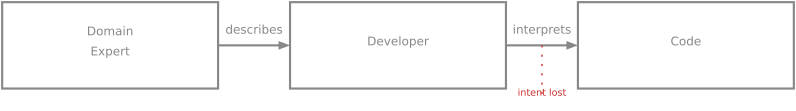
\includegraphics{pcd-workflow-today.png}

Every handoff loses information.\\
Requirements get simplified.\\
Misunderstandings go undetected.
\end{column}

\begin{column}{0.5\textwidth}
\textbf{With PCD}

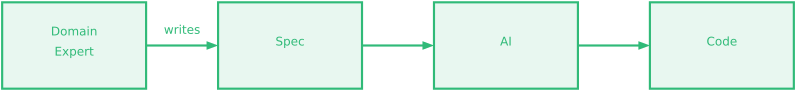
\includegraphics{pcd-workflow-pcd.png}

The cardiologist specifies\\
the device behaviour directly.

No interpreter in the middle.
\end{column}
\end{columns}
\end{frame}

\begin{frame}{And: formal verification is available}
\protect\hypertarget{and-formal-verification-is-available}{}
The LLM translation is probabilistic --- we do not claim otherwise.

\bigskip

For components that \textbf{require} stronger guarantees:

\bigskip

\begin{columns}[T]
\begin{column}{0.6\textwidth}
Lean 4, F*, or Dafny can be added~ as an \textbf{optional verification
layer} ---~ without changing the specification format.

The spec stays the same.~ The verification path is a template choice.
\end{column}

\begin{column}{0.4\textwidth}
\begin{itemize}
\tightlist
\item
  memory safety by construction
\item
  formal proofs of invariants
\item
  state machine correctness
\item
  ISO 26262 / DO-178C evidence
\end{itemize}
\end{column}
\end{columns}
\end{frame}

\begin{frame}[fragile]{Proof: pcd-lint}
\protect\hypertarget{proof-pcd-lint}{}
\texttt{pcd-lint} --- the specification validator --- was~
\textbf{specified and generated using PCD itself.}

Zero hand-written implementation code.

\bigskip

Tested across multiple AI models,~ three continents, one result:

\bigskip

\begin{center}
\Large Every model resolved Go from the template\\
\large without being told.
\end{center}
\end{frame}

\begin{frame}
\end{frame}

\hypertarget{how}{%
\section{How}\label{how}}

\begin{frame}[fragile]{The workflow}
\protect\hypertarget{the-workflow}{}
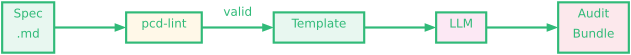
\includegraphics[width=\textwidth,height=3cm]{pcd-workflow.png}

\begin{enumerate}
\tightlist
\item
  Domain expert writes a spec (or AI interviews them)
\item
  \texttt{pcd-lint} validates structure
\item
  Deployment template resolves the language
\item
  LLM translates spec \textrightarrow{} code + audit bundle
\end{enumerate}
\end{frame}

\begin{frame}{Language is never your problem}
\protect\hypertarget{language-is-never-your-problem}{}
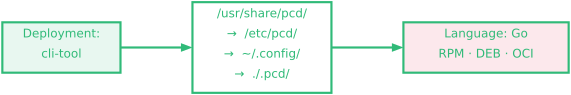
\includegraphics[width=\textwidth,height=3cm]{pcd-resolution.png}

The spec declares \textbf{what} and \textbf{where} (deployment context).

The template resolves \textbf{language, packaging, conventions}.

A spec written today is valid if the organisation\\
switches from Go to Rust in 2045 --- \textbf{no spec change needed}.
\end{frame}

\begin{frame}{The audit bundle}
\protect\hypertarget{the-audit-bundle}{}
\begin{columns}[T]
\begin{column}{0.5\textwidth}
Every translation produces:

\begin{itemize}
\tightlist
\item
  specification (human-reviewable)
\item
  generated source code
\item
  packaging artifacts (RPM, DEB, OCI)
\item
  independent test suite
\item
  translation report
\item
  workflow diagram (Pikchr)
\item
  metadata + hashes
\end{itemize}
\end{column}

\begin{column}{0.5\textwidth}
Designed for:

\begin{itemize}
\tightlist
\item
  ISO 26262 (automotive)
\item
  DO-178C (aviation)
\item
  IEC 62304 (medical)
\item
  Common Criteria EAL4+
\item
  EU Cyber Resilience Act
\end{itemize}
\end{column}
\end{columns}
\end{frame}

\begin{frame}[fragile]{Getting started}
\protect\hypertarget{getting-started}{}
\begin{columns}[T]
\begin{column}{0.5\textwidth}
\textbf{Write a spec (no format knowledge needed):}

\begin{Shaded}
\begin{Highlighting}[]
\CommentTok{\# AI interviews the domain expert:}
\ExtensionTok{ollama}\NormalTok{ run llama3.2 }\DataTypeTok{\textbackslash{}}
  \StringTok{"}\VariableTok{$(}\FunctionTok{cat}\NormalTok{ prompts/interview{-}prompt.md}\VariableTok{)}\StringTok{"}
\end{Highlighting}
\end{Shaded}

Then validate:

\begin{Shaded}
\begin{Highlighting}[]
\ExtensionTok{pcd{-}lint}\NormalTok{ myspec.md}
\end{Highlighting}
\end{Shaded}
\end{column}

\begin{column}{0.5\textwidth}
\textbf{Translate to code:}

\begin{Shaded}
\begin{Highlighting}[]
\CommentTok{\# mcphost with the translator prompt}
\CommentTok{\# reads template + spec,}
\CommentTok{\# produces code + audit bundle}
\end{Highlighting}
\end{Shaded}

\bigskip

Everything in the repo:\\
\textbf{github.com/mge1512/pcd}
\end{column}
\end{columns}
\end{frame}

\hypertarget{the-specification-1}{%
\section{The specification}\label{the-specification-1}}

\begin{frame}[fragile]{Spec sections}
\protect\hypertarget{spec-sections}{}
\begin{columns}[T]
\begin{column}{0.45\textwidth}
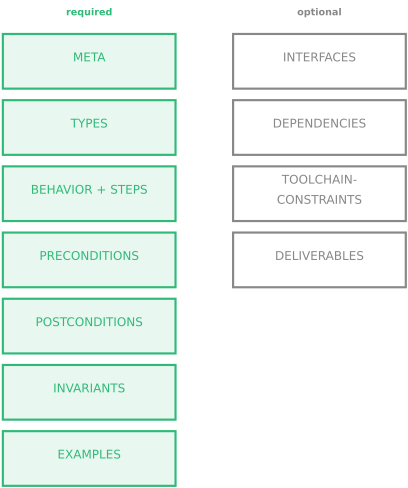
\includegraphics[width=\textwidth,height=6cm]{pcd-spec-sections.png}
\end{column}

\begin{column}{0.55\textwidth}
\texttt{pcd-lint} validates structure\\
before any translation begins.

\bigskip

\textbf{Key constraints:}

\begin{itemize}
\tightlist
\item
  BEHAVIOR must include \texttt{STEPS:}
\item
  INVARIANTS carry \texttt{{[}observable{]}}\\
  or \texttt{{[}implementation{]}} tags
\item
  EXAMPLES must cover error paths
\item
  No programming language in spec
\end{itemize}
\end{column}
\end{columns}
\end{frame}

\begin{frame}[fragile]{BEHAVIOR in depth}
\protect\hypertarget{behavior-in-depth}{}
\begin{columns}[T]
\begin{column}{0.52\textwidth}
\begin{Shaded}
\begin{Highlighting}[]
\FunctionTok{\#\# BEHAVIOR: shutdown}
\NormalTok{Constraint: required}
\NormalTok{INPUTS:}
\NormalTok{  vm: VirtualMachine}
\NormalTok{PRECONDITIONS:}
\SpecialStringTok{  {-} }\NormalTok{vm.state = Running}
\NormalTok{STEPS:}
\SpecialStringTok{  1. }\NormalTok{Send shutdown signal.}
\SpecialStringTok{  2. }\NormalTok{Record shutdown{-}start time.}
\NormalTok{     MECHANISM: do NOT block;}
\NormalTok{     requeue immediately.}
\SpecialStringTok{  3. }\NormalTok{On re{-}entry: check elapsed.}
\NormalTok{     If \textgreater{} timeout: Destroy(vm).}
\NormalTok{POSTCONDITIONS:}
\SpecialStringTok{  {-} }\NormalTok{vm.state = Stopped}
\end{Highlighting}
\end{Shaded}
\end{column}

\begin{column}{0.48\textwidth}
\texttt{STEPS} = the algorithm,\\
not just the contract.

\bigskip

\texttt{MECHANISM:} = where the\\
\emph{how} matters for correctness.

\bigskip

\texttt{Constraint:} field:

\begin{itemize}
\tightlist
\item
  \texttt{required} --- always implement
\item
  \texttt{supported} --- preset activates it
\item
  \texttt{forbidden} --- never implement
\end{itemize}
\end{column}
\end{columns}
\end{frame}

\begin{frame}[fragile]{INTERFACES: testable abstractions}
\protect\hypertarget{interfaces-testable-abstractions}{}
\begin{Shaded}
\begin{Highlighting}[]
\FunctionTok{\#\# INTERFACES}

\NormalTok{Transport \{}
\NormalTok{  required{-}methods:}
\NormalTok{    Connect(ctx, spec) {-}\textgreater{} (Session, error)}
\NormalTok{  implementations{-}required:}
\NormalTok{    production:  RealTransport}
\NormalTok{    test{-}double: FakeTransport \{}
\NormalTok{      configurable: ConnectErr, Sessions}
\NormalTok{    \}}
\NormalTok{\}}
\end{Highlighting}
\end{Shaded}

\bigskip

Independent tests use \textbf{only} declared test doubles.\\
\texttt{go\ test\ ./independent\_tests/} runs without any live service.
\end{frame}

\begin{frame}
\end{frame}

\hypertarget{templates-and-translation}{%
\section{Templates and translation}\label{templates-and-translation}}

\begin{frame}{Deployment templates}
\protect\hypertarget{deployment-templates}{}
\begin{columns}[T]
\begin{column}{0.5\textwidth}
Templates encode \textbf{everything} the spec does not:

\begin{itemize}
\tightlist
\item
  target language + alternatives
\item
  binary type, packaging formats
\item
  CLI conventions
\item
  security constraints
\item
  TYPE-BINDINGS
\item
  delivery phases (EXECUTION)
\item
  compile gate
\end{itemize}
\end{column}

\begin{column}{0.5\textwidth}
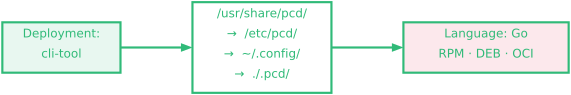
\includegraphics[width=\textwidth,height=3cm]{pcd-resolution.png}

\bigskip

One preset file changes\\
language for the whole project.

The spec is untouched.
\end{column}
\end{columns}
\end{frame}

\begin{frame}[fragile]{TYPE-BINDINGS: no translator discretion}
\protect\hypertarget{type-bindings-no-translator-discretion}{}
Template excerpt:

\begin{Shaded}
\begin{Highlighting}[]
\FunctionTok{\#\# TYPE{-}BINDINGS}
\NormalTok{| Spec type  | LANGUAGE=Go           |}
\NormalTok{|{-}{-}{-}{-}{-}{-}{-}{-}{-}{-}{-}{-}|{-}{-}{-}{-}{-}{-}{-}{-}{-}{-}{-}{-}{-}{-}{-}{-}{-}{-}{-}{-}{-}{-}{-}|}
\NormalTok{| Duration   | metav1.Duration       |}
\NormalTok{| Timestamp  | metav1.Time           |}
\NormalTok{| Condition  | metav1.Condition      |}
\NormalTok{| List}\KeywordTok{\textless{}T\textgreater{}}\NormalTok{    | []T                   |}
\end{Highlighting}
\end{Shaded}

\bigskip

Without TYPE-BINDINGS: one translator produces \texttt{string},\\
another produces \texttt{metav1.Duration} --- incompatible at the API
level.

\bigskip

With TYPE-BINDINGS: \textbf{deterministic, language-specific types} ---
applied\\
mechanically, not by translator judgement.
\end{frame}

\begin{frame}[fragile]{The translation phases}
\protect\hypertarget{the-translation-phases}{}
\begin{columns}[T]
\begin{column}{0.4\textwidth}
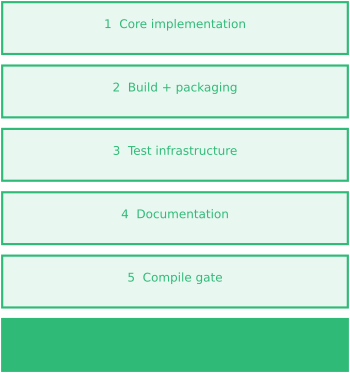
\includegraphics[width=\textwidth,height=5.5cm]{pcd-translation-phases.png}
\end{column}

\begin{column}{0.6\textwidth}
Defined in the template's\\
\texttt{\#\#\ EXECUTION} section ---\\
\textbf{not} in the prompt.

\bigskip

\textbf{Resume logic:} partial runs\\
restart from the first missing file.

\bigskip

\textbf{Compile gate} is language-specific:

\begin{Shaded}
\begin{Highlighting}[]
\ExtensionTok{go}\NormalTok{ mod tidy   }\CommentTok{\# direct deps only}
              \CommentTok{\# no fabricated versions}
\ExtensionTok{go}\NormalTok{ build ./...}
\end{Highlighting}
\end{Shaded}

\bigskip

\texttt{TRANSLATION\_REPORT.md} is\\
\textbf{always last} --- its presence\\
signals a complete run.
\end{column}
\end{columns}
\end{frame}

\begin{frame}
\end{frame}

\hypertarget{tooling}{%
\section{Tooling}\label{tooling}}

\begin{frame}[fragile]{pcd-lint}
\protect\hypertarget{pcd-lint}{}
\begin{columns}[T]
\begin{column}{0.55\textwidth}
\textbf{What it validates:}

\begin{itemize}
\tightlist
\item
  required sections present
\item
  META fields + SPDX license
\item
  deployment template resolves
\item
  BEHAVIOR has STEPS
\item
  INVARIANTS have tags
\item
  EXAMPLES cover error paths
\item
  Constraint: field values
\item
  cross-section consistency
\end{itemize}
\end{column}

\begin{column}{0.45\textwidth}
\textbf{Self-hosting:}

\texttt{pcd-lint} was specified and\\
generated using PCD itself.

\bigskip

Running \texttt{pcd-lint} against\\
its own spec passes --- the\\
paradigm validates itself.

\bigskip

\begin{Shaded}
\begin{Highlighting}[]
\ExtensionTok{pcd{-}lint}\NormalTok{ myspec.md}
\ExtensionTok{pcd{-}lint}\NormalTok{ strict=true myspec.md}
\ExtensionTok{pcd{-}lint}\NormalTok{ list{-}templates}
\end{Highlighting}
\end{Shaded}
\end{column}
\end{columns}
\end{frame}

\begin{frame}[fragile]{Translation confidence}
\protect\hypertarget{translation-confidence}{}
Every \texttt{TRANSLATION\_REPORT.md} includes:

\bigskip

\begin{longtable}[]{@{}
  >{\raggedright\arraybackslash}p{(\columnwidth - 6\tabcolsep) * \real{0.1910}}
  >{\raggedright\arraybackslash}p{(\columnwidth - 6\tabcolsep) * \real{0.1461}}
  >{\raggedright\arraybackslash}p{(\columnwidth - 6\tabcolsep) * \real{0.4270}}
  >{\raggedright\arraybackslash}p{(\columnwidth - 6\tabcolsep) * \real{0.2360}}@{}}
\toprule()
\begin{minipage}[b]{\linewidth}\raggedright
EXAMPLE
\end{minipage} & \begin{minipage}[b]{\linewidth}\raggedright
Confidence
\end{minipage} & \begin{minipage}[b]{\linewidth}\raggedright
Verification method
\end{minipage} & \begin{minipage}[b]{\linewidth}\raggedright
Unverified claims
\end{minipage} \\
\midrule()
\endhead
vm-start & High & \texttt{TestVMStart} --- FakeSession &
\begin{minipage}[t]{\linewidth}\raggedright
libvirt UUID format
\end{minipage} \\
graceful-stop & Medium & \texttt{TestGracefulStop} pass 1 only & timeout
path \\
host-ready & Low & none & entire sequence \\
\bottomrule()
\end{longtable}

\bigskip

\begin{itemize}
\tightlist
\item
  \textbf{High} = named test in \texttt{independent\_tests/} passes
  without live services
\item
  \textbf{Medium} = partial test coverage
\item
  \textbf{Low} = reasoning only --- no test
\end{itemize}

\bigskip

Unverified claims must be listed \textbf{explicitly}. Never silently
omitted.
\end{frame}

\begin{frame}[fragile]{Large projects}
\protect\hypertarget{large-projects}{}
\begin{columns}[T]
\begin{column}{0.55\textwidth}
\textbf{Architect defines interfaces first:}

\begin{Shaded}
\begin{Highlighting}[]
\FunctionTok{\#\# INTERFACE}
\NormalTok{EXPORTS:}
\NormalTok{  TYPES:  Account, TransferResult}
\NormalTok{  BEHAVIOR: transfer}
\NormalTok{  INVARIANTS:}
\SpecialStringTok{    {-} }\NormalTok{GLOBAL: balance \textgreater{}= 0}
\end{Highlighting}
\end{Shaded}

\bigskip

Component specs declare imports:

\begin{Shaded}
\begin{Highlighting}[]
\AnnotationTok{Imports:}
\SpecialStringTok{  {-} }\NormalTok{account{-}svc: ./account.md}
\NormalTok{                 \#INTERFACE@\textgreater{}=1.2.0}
\end{Highlighting}
\end{Shaded}
\end{column}

\begin{column}{0.45\textwidth}
\textbf{Rules:}

\begin{itemize}
\tightlist
\item
  interfaces before implementation
\item
  build order = topological sort
\item
  no circular dependencies
\item
  component fits in one LLM\\
  context window
\end{itemize}

\bigskip

\textbf{pcd-lint v2} (planned):\\
validates full project graph ---\\
imports, circular deps,\\
interface versioning.
\end{column}
\end{columns}
\end{frame}

\begin{frame}[fragile]{mcp-server-pcd}
\protect\hypertarget{mcp-server-pcd}{}
\begin{columns}[T]
\begin{column}{0.45\textwidth}
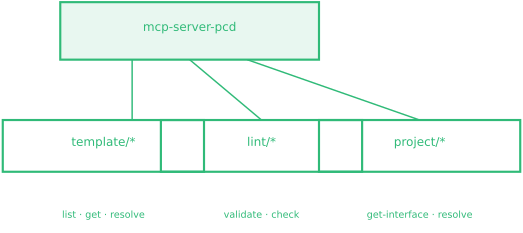
\includegraphics[width=\textwidth,height=4cm]{pcd-mcp-server.png}
\end{column}

\begin{column}{0.55\textwidth}
Any MCP-capable host connects directly:

\begin{itemize}
\tightlist
\item
  \textbf{mcphost} (CLI)
\item
  \textbf{VS Code} with Copilot
\item
  \textbf{Claude Desktop}
\item
  custom agents
\end{itemize}

\bigskip

Preset layering server-side:\\
vendor \textrightarrow{} \texttt{/etc/pcd-server/} \textrightarrow{}
team \textrightarrow{} user

\bigskip

The LLM is the wizard.\\
The server is the data layer.
\end{column}
\end{columns}
\end{frame}

\hypertarget{update-april-to-september-2026}{%
\section{Update: April to September
2026}\label{update-april-to-september-2026}}

\begin{frame}[fragile]{Whitepaper 0.3.22 to 0.4.6: what changed}
\protect\hypertarget{whitepaper-0.3.22-to-0.4.6-what-changed}{}
\begin{longtable}[]{@{}
  >{\raggedright\arraybackslash}p{(\columnwidth - 2\tabcolsep) * \real{0.5000}}
  >{\raggedright\arraybackslash}p{(\columnwidth - 2\tabcolsep) * \real{0.5000}}@{}}
\toprule()
\begin{minipage}[b]{\linewidth}\raggedright
Area
\end{minipage} & \begin{minipage}[b]{\linewidth}\raggedright
Change
\end{minipage} \\
\midrule()
\endhead
Composition & \texttt{Includes:} merges shared specs into a host spec;
merged spec hash; RULE-19 to RULE-21 \\
TYPES & Tabular TYPE grammar, closed cell vocabularies; RULE-22 to
RULE-25; JSON Schema emission \\
Provenance & Reports record a SHA-256 for every translation input, not
the spec hash alone \\
Verification & Tests-first enforced structurally; roles renamed to
translator / test-author \\
Templates & 14 deployment templates, was 9: abap-report, cockpit-module,
kubectl-style-cli, library, spack-package added \\
Tooling & \texttt{pcd-slice} shipped; \texttt{libpcd} and
\texttt{pcd-emit-types} specified \\
\bottomrule()
\end{longtable}

\bigskip

The reproducibility unit is now a tuple: spec + resolved language +
hints and template set.\\
The spec hash attests intended behaviour; it does not alone determine
the binary.
\end{frame}

\begin{frame}[fragile]{pcd-lint: from 17 to 25 rules - and one engine}
\protect\hypertarget{pcd-lint-from-17-to-25-rules---and-one-engine}{}
\textbf{Rules added since April:}

\begin{itemize}
\tightlist
\item
  RULE-18: generated output embeds the correct spec hash
  (\texttt{check-report=true})
\item
  RULE-19 to RULE-21: composition - paths resolve, no name collisions,
  inclusion graph acyclic
\item
  RULE-22 to RULE-25: tabular TYPES - structure, cell vocabulary,
  references, lifecycle
\end{itemize}

\bigskip

\textbf{Consolidation into one engine:}

\begin{itemize}
\tightlist
\item
  Every rule is written once, in \texttt{tools/shared/spec/}, and
  composed via \texttt{Includes:} into \texttt{libpcd}
\item
  \texttt{pcd-lint}, \texttt{pcd-emit-types} (TYPE tables to JSON
  Schema), and \texttt{mcp-server-pcd} are thin front ends binding to
  that engine
\item
  Lint parity between CLI and MCP holds by construction, not by copy
  discipline
\end{itemize}

\bigskip

Status: \texttt{pcd-lint} shipped - Go, RPM and DEB from the Open Build
Service.\\
\texttt{libpcd} and \texttt{pcd-emit-types}: specified, translation
pending.
\end{frame}

\begin{frame}[fragile]{pcd-slice: bundles instead of full-spec reads}
\protect\hypertarget{pcd-slice-bundles-instead-of-full-spec-reads}{}
A translation reads the spec many times - per milestone, per role.\\
One full pass over a 41-BEHAVIOR production spec is on the order of 70K
tokens.

\bigskip

\texttt{pcd-slice} derives the semantic form once, deterministically:

\begin{itemize}
\tightlist
\item
  One preamble with what every bundle shares: version, intro, full
  TYPES, global invariants.\\
  Byte-identical across bundles, so it becomes a cacheable prompt
  prefix.
\item
  One bundle per BEHAVIOR: the block verbatim, its examples, its
  invariants, its hints, its type closure by name
\end{itemize}

\bigskip

\begin{itemize}
\tightlist
\item
  Every emitted file records the SHA-256 of its sources;
  \texttt{pcd-slice\ check} detects stale bundles
\item
  The source spec is never modified: bundles are build output,
  regeneratable
\item
  \texttt{skills/pcd-translate} guards a session: translation reads
  bundles, never the spec
\end{itemize}

\bigskip

Shipped: Go, single static binary, standard library only, packaged via
OBS.\\
Read-cost reduction on production specs: typically 50 to 65 percent,
before caching.
\end{frame}

\begin{frame}[fragile]{The workflow, updated}
\protect\hypertarget{the-workflow-updated}{}
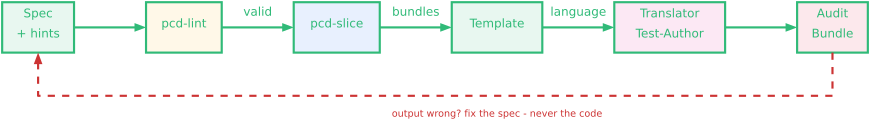
\includegraphics[width=1\textwidth,height=\textheight]{pcd-workflow-full.png}

\begin{enumerate}
\tightlist
\item
  Domain expert writes the spec, or an AI interview produces it
\item
  \texttt{pcd-lint} validates: 25 rules, before any translation
\item
  \texttt{pcd-slice} derives the preamble and the per-BEHAVIOR bundles
\item
  The deployment template resolves language, packaging, conventions
\item
  Translator and test-author produce code, tests, and the audit bundle
\end{enumerate}

If the output is wrong: fix the spec and regenerate. The code is never
touched.
\end{frame}

\end{document}
